\documentclass[a4]{article} 
\usepackage[czech]{babel} 
\usepackage[utf8]{inputenc} 
\usepackage{caption}
\usepackage{subcaption}
\usepackage{a4wide} 
\usepackage{amsmath,amsfonts,amssymb,amsthm}
\usepackage{graphicx}
\graphicspath{ {images/} }
\usepackage{float}
\usepackage{wrapfig}
\floatstyle{boxed} 
\restylefloat{figure}
\usepackage{geometry}
\usepackage{tikz,pgfplots} 
 \geometry{
 a4paper,
 left=40mm,
 top=25mm,
 bottom=25mm,
 right=25mm
 }



%TODO pridat geometry a udelat spravne okraje 
\begin{document} 
 
%titulni strana 
\begin{titlepage} 
\begin{center} 
{\huge\textsc{Gymnázium Jana Keplera}\\}
{\large{Parléřova 2, Praha 6}}\\
{\large{obor vzdělání Gymnázium 79-41-K/81}\\[5cm]} 
{\Large{Maturitní práce z~informatiky}\\[0.2cm]}
{\Huge{Vývoj chůze pomocí\\neuroevolučních algoritmů}}\\\vfill
{\Large{Jan Bouček}\\} 
{\large{vedoucí práce: Ing. Tomáš Obdržálek}\\} 
{\large{Praha 2017}} 
\end{center} 
\end{titlepage} 
 
%prohlaseni 
\newpage 
Prohlašuji, že jsem jediným autorem této maturitní práce a všechny citace, použitá literatura a další zdroje jsou v~práci uvedené. Tímto dle zákona 121/2000 Sb. (tzv. Autorský zákon) ve znění pozdějších předpisů uděluji bezúplatně škole Gymnázium Jana Keplera, Praha 6, Parléřova 2, oprávnění k~výkonu práva na rozmnožování díla (§~13) a práva na sdělování díla veřejnosti (§~18) na dobu časově neomezenou a bez omezení územního rozsahu.\\[0.7cm] 
\vspace{10cm} 
{\large{V Praze dne 24. 3. 2017} \hfill Jan Bouček} 
%anotace 
\newpage 
\tableofcontents
\newpage
%TODO zrušit mezeru na začátku 
{\Large\textbf{Anotace}\par}
Jeden z~problémů moderní robotiky je chůze, čehož se tato práce na rozdíl od konvenčních metod snaží dosáhnout pomocí strojového učení, konkrétně neuroevolučního algoritmu s~nepřímým kódováním. Ten za pomoci techniky HyperNEAT generuje simulaci primitivního mozku, který chůzi robota ovládá.\par 

{\Large\textbf{Annotation}\par}
One of the problems in modern robotics is robotic walking, which in this paper, unlike conventional methods, is achieved by machine learning, specifically using a neuroevolutionary algorithm with indirect encoding. The algorithm uses the HyperNEAT technique to generate a simulation of a primitive brain, which controls the gait of the robot.\par  

%samotna prace 
\title{Vývoj chůze pomocí neuroevolučních algoritmů} 
\author{Jan Bouček} 
\date{} 
\maketitle 
 
\section{Úvod} 
Jeden z~cílů dnešní robotiky je konstruovat roboty, kteří jsou všestranně využitelní díky své mobilitě. Toho lze dosáhnout různými způsoby, pro svou jednoduchost se často používá jízda, která však neumožňuje spolehlivé zdolávání členitého terénu, nebo pohyb přímo ve strukturách stavěných člověkem, zejména pak zdolávání schodů.\par
Tato práce se inspiruje čtyřnohými kráčivými roboty firmy Boston Dynamics\cite{bostondynamics}, kteří dosahují stabilní chůze exaktními metodami.\cite{bdpaper} Podobné chůze by mělo být možné dosáhnout i pomocí organičtějších metod. Neuroevoluční algoritmy dokážou nabídnout přirozené řešení i velmi komplexních problémů, či dokonce znovuobjevit řešení, které v~přírodě už existuje, proto je možné generovat čtyřnohý pohyb i tímto způsobem.\cite{clunegait}\par
Cílem projektu pak je dosáhnout podobnou metodou stabilní, vzpřímené a repetitivní chůze vpřed na simulaci čtyřnohého robota.
 
\section{Teorie}
Chůzi lze definovat jakožto sérii stavů kráčivého tělesa, kde každý stav lze zjednodušit jako soubor informací popisujících jednotlivé pohyblivé prvky robota. V~rámci tohoto projektu budeme pracovat s~dvojrozměrnou simulací čtyřnohého robota, jehož každá noha je ovládána dvěma klouby. Stav robota tak lze vystihnout jako osmirozměrný vektor $\vec{s}$. Hledáme pak ovladač robota, který pro každý stav malezne osmirozměrný vektor $\vec{\omega}$, tem každému kloubu určuje úhlovou rychlost.
\subsection{Evoluční algoritmy}
Evoluční algoritmy jsou metodou, která dokáže mnohnásobnou selekcí, mutací a kombinací různých řešení postupně vyvíjet postupně lepší řešení. K~tomu potřebuje funkci, která dokáže každé řešení ohodnotit, tzv. \emph{fitness funkci}. V~našem případě hodnotíme maximální vzdálenost robota od počátku směrem do kladných hodnot $x$, a vzhledem k~tomu, že cílem je chůze vzpřímená, tak u~každého řešení, ve kterém některý článek robota klesne svou výškou těžiště pod experimentálně zjištěnou hodnotu $Y_{min}$, nastavíme výslednou \emph{fitness} ovladače na \emph{0}.\par
Podobně jako v~přírodě, evoluční algoritmus si udržuje \emph{populaci} řešení. V~každém kroku ohodnotí výše zmíněnou funkcí všechny \emph{živočichy}, kteří jsou pak podle své úspěšnosti rozmnoženi (pohlavně, či nepohlavně) a zmutováni. Tento proces je podrobněji popsán v~následující sekci.
\subsection{Neuroevoluce}
Neuroevoluční algoritmy jsou specifickou kategorií, která se zabývá trénováním umělých neuronových sítí, anglicky \emph{Artificial Neural Network} (ANN), které jsou abstraktním příblížením dějů v~mozku, měly by být tedy schopné sloužit i jako ovladač projektovaného robota. Jejich struktura je popsána níže.
\subsubsection{Neuronové sítě}
Základní stavební jednotkou neuronové sítě je \emph{neuron}, ten je výpočetní jednotkou, která přijímá data ve formě spojů (z~biologického hlediska \emph{dendrity}) s~dalšími neurony. Pro každý z~nich má nastavenou \emph{váhu} (anglicky \emph{weight}), která slouží jednoduše jako koeficient, který ovlivňuje \uv{důležitost} konkrétního spoje.\par
Výstupem, který pak mohou použít další neurony, je výsledek \emph{aktivační funkce} skalárního součinu hodnot napojených neuronů a příslušných vah\cite{neuron}:
\begin{center}$y_k=\phi(\sum_{j=0}^m w_{kj}\cdot x_j)$,\end{center}
kde $w$ je váha hodnoty neuronu $x$ a $\phi$ aktivační funkce.\par
Neurony pak lze tímto způsobem zapojovat do komplexnich sítí, kde hodnotu některých neuronů určujeme manuálně -- považujeme je za \emph{vstupy} sítě a u~některých neuronů zjišťujeme hodnoty, které fungují jako \emph{výstupy} sítě.
\subsubsection{NEAT}
\emph{Neuroevolution of augmenting topologies}\cite{neat} (NEAT) je metodou, která definuje jeden ze způsobů, kterými lze vyvíjet neuronové sítě pomocí evolučního algoritmu. Revoluční ideou tohoto systému je způsob, kterým zapisuje neuronové sítě, jakožto \emph{živočicha}.\par
Tento systém každou neuronovou síť popisuje jako ohodnocený graf pomocí dvou seznamů \emph{genů} -- seznamu vrcholů a seznamu hran. Každému vrcholu a hraně přisuzuje číselné identifikátory, pomocí kterých je dokáže přehledně propojovat a udržovat přehled o~tom, kteří jedinci jsou si \uv{geneticky} podobní.\par
Stanley a Miikkulainen díky tomu zavádí i proces \emph{speciace}, který ještě před rozmnožováním roztřídí jedince na různé \emph{druhy} podle příbuznosti tak, aby se spolu křížily jen sítě s~menšími rozdíly. Každý druh je pak ohodnocen svojí průměrnou hodnotou fitness, pomocí které se určí počet potomků v~další generaci daného druhu.\par
Při procesu rozmnožování je z~každého druhu vybrána \emph{silnější} část, ze které se vytvoří požadovaný počet potomků, z~nichž každý může vzniknout křížením -- většinu genů zdědí po silnějším rodiči, ale část od slabšího, nebo bez křížení, kdy se jedinec pouze zkopíruje do další generace.\par
Pak na všech potomcích proběhnou mutace, přičemž je náhodně rozhodnuto, které z~druhů mutací na nich proběhnou, Stanley a Miikkulainen jich popisují hned několik:
\begin{itemize}
\item{přidání nové hrany do sítě}
\item{rozdělení hrany na dvě hrany s~novým neuronem uprostřed}
\item{změna všech vah o~malou hodnotu, nebo na náhodnou hodnotu}
\end{itemize}
V~tomto projektu je použito ještě několik dalších mutačních operátorů:
\begin{itemize}
\item{aktivace/deaktivace jedné hrany}
\item{změna jedné váhy na náhodnou hodnotu}
\item{změna jedné váhy o~maximálně $\pm 5\%$}
\end{itemize}
Díky této malé úpravě dokáže algoritmus ladit neuronovou síť v~mírně detailnějším měřítku.\par
Po zmutování jsou všichni potomci prohlášeni za současnou generaci a algoritmus pokračuje znovu hodnocením jedinců.
\subsection{CPPN-NEAT}
Tím, že v~NEAT algoritmu umožníme každému neuronu využívat jinou aktivační funkci, můžeme dosáhnout tvorby sítí, které jsou dobře uzpůsobené ke generování fyzické geometrie živočichů. Metoda CPPN-NEAT\cite{cppn-neat} využívá různých vlastností funkcí -- symetrie, repetice apod. tak, že~průchodem celou sítí jsou výsledná data nakombinována pomocí komplexní složené funkce, která si uchováva všechny tyto vlastnosti.\par
Pokud například vytvoříme CPPN síť s~dvěma vstupy -- souřadnicemi $x$ a $y$ s~jedním výstupem, získáme dvojrozměrné útvary (viz~obr.~1), které mají velmi blízko k~fyzickému rozložení v~reálných živočiších, např. dokáže nakombinovat repetici s~variací a generovat útvary podobné prstům ruky nebo pomocí symetrie a variace útvar podobný lidskému oku (viz obr. 1b)\par
V~samotném algoritmu stačí jen při tvoření nových neuronů určit náhodnou aktivační funkci a přidat mutační operátor, který změní funkci u~náhodného neuronu.\par

%https://en.wikibooks.org/wiki/LaTeX/Floats,_Figures_and_Captions#Subfloats
\begin{figure}
    \centering
    \begin{subfigure}[b]{0.3\textwidth}
        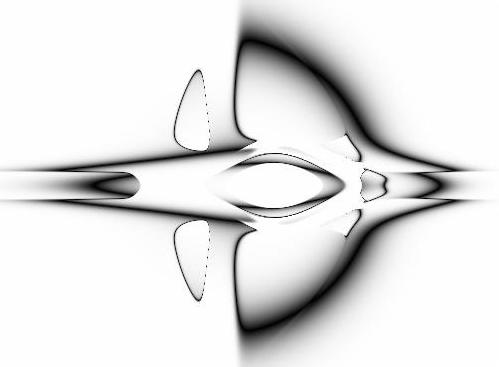
\includegraphics[width=\textwidth]{cppn1}
        \caption{symetrie}
        \label{fig:sym}
    \end{subfigure}
    ~ 
    \begin{subfigure}[b]{0.3\textwidth}
        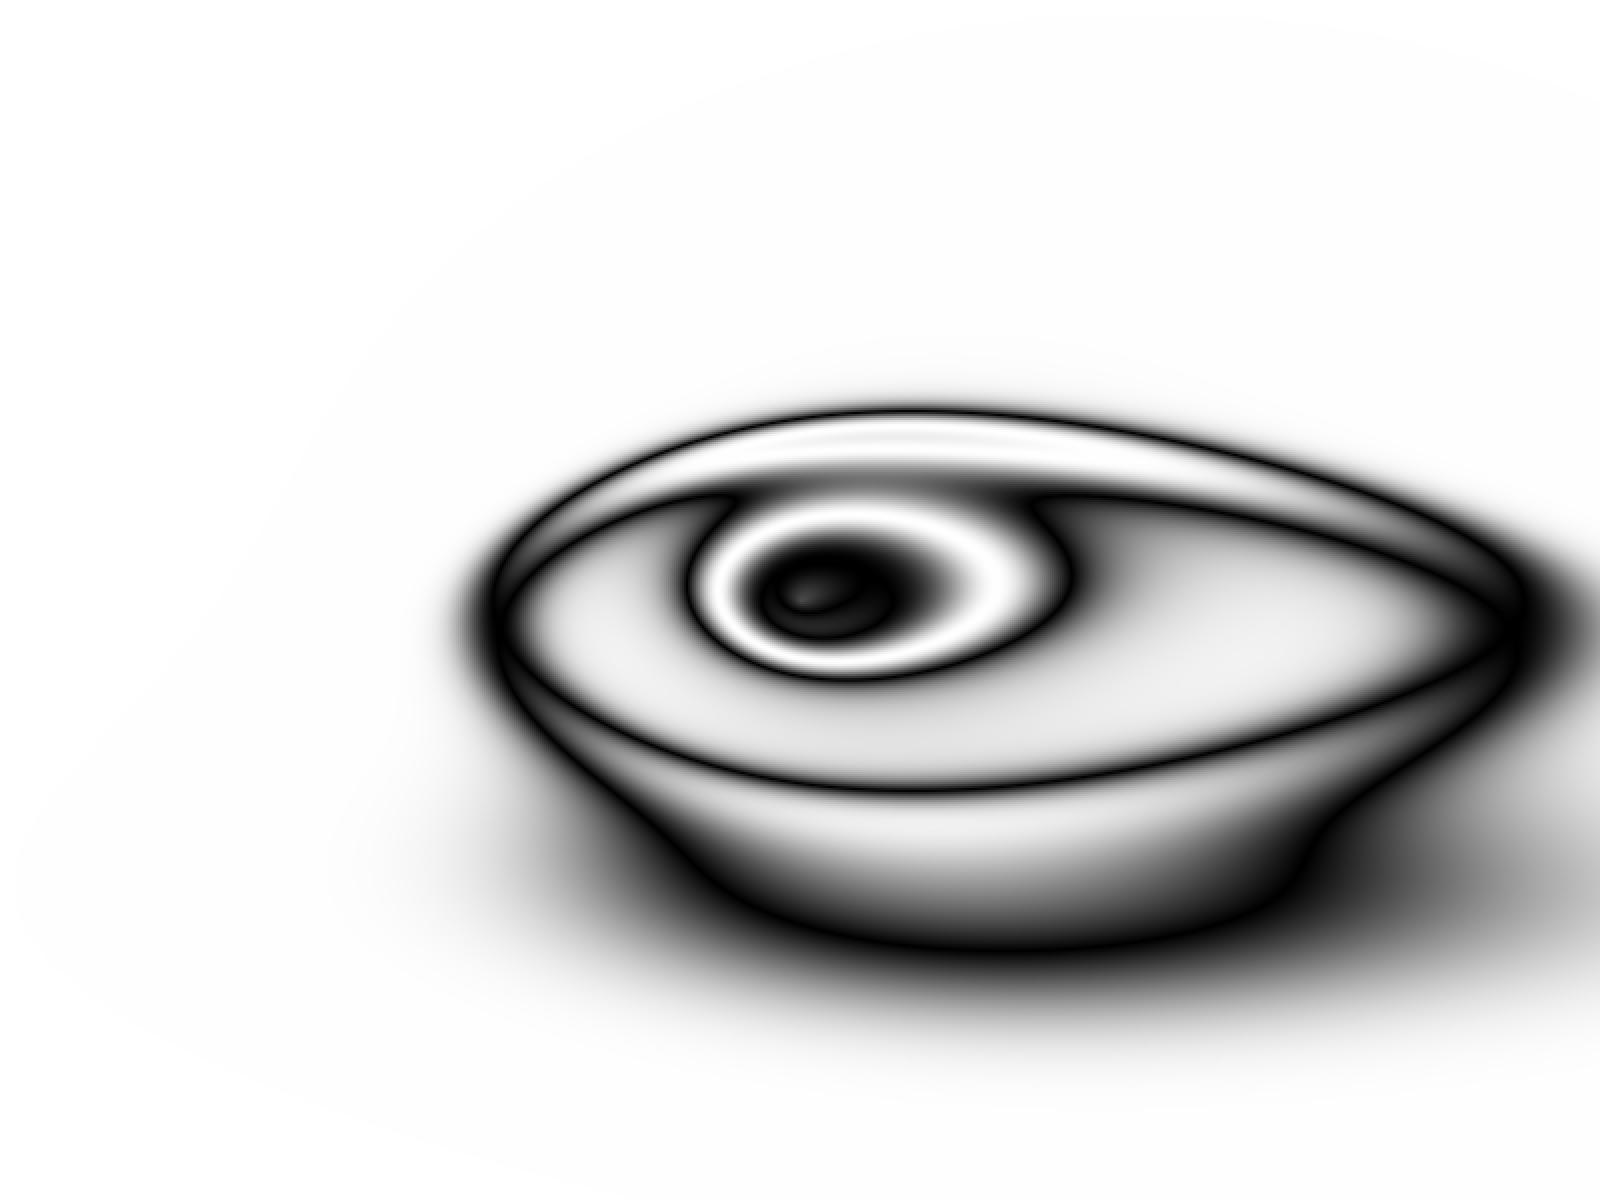
\includegraphics[width=\textwidth]{cppn2}
        \caption{nedokonalá symetrie}
        \label{fig:imperfectsym}
    \end{subfigure}
    ~ 
    \begin{subfigure}[b]{0.3\textwidth}
        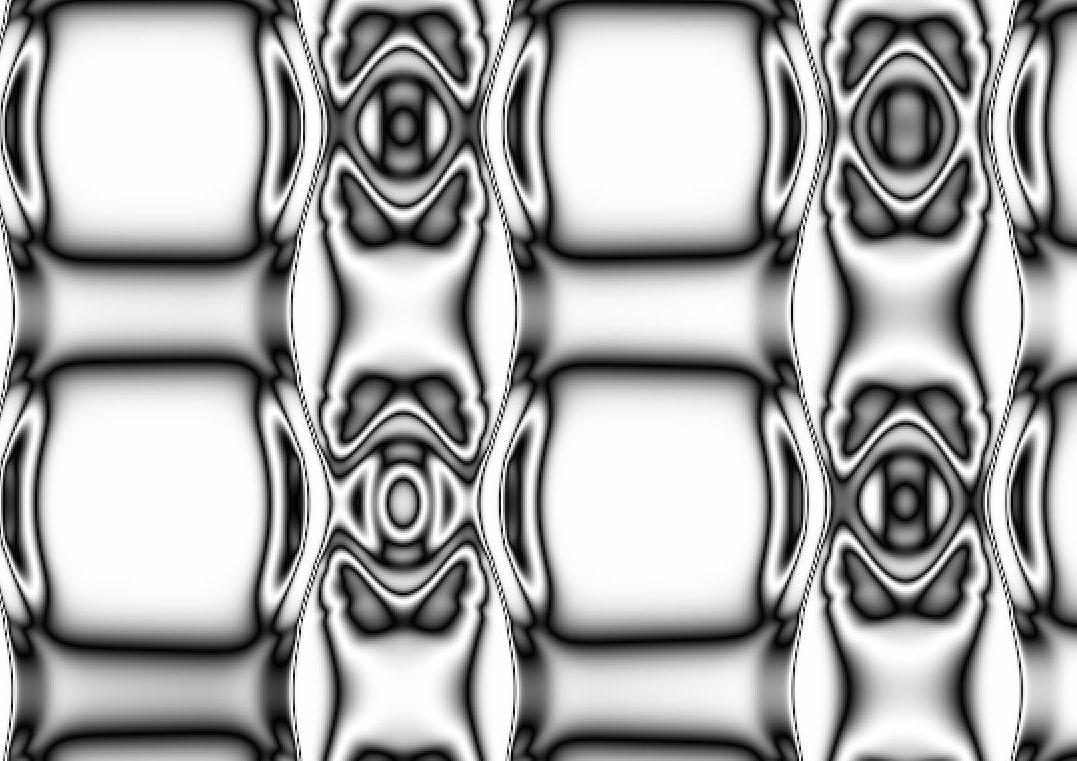
\includegraphics[width=\textwidth]{cppn3}
        \caption{repetice s~variací}
        \label{fig:repvar}
    \end{subfigure}
    \caption{tvary vygenerované pomocí CPPN-NEAT, převzato\cite{hyperneat}}\label{fig:cppn}
\end{figure}
\subsection{HyperNEAT}
Technika HyperNEAT\cite{hyperneat} využívá CPPN sítě ke generování čtyřrozměrného prostoru, který ve výsledku slouží jako definice vah v~další neuronové síti.\par
To znamená, že generujeme CPPN síť, která má čtyři vstupy -- $x_1$, $y_1$, $x_2$, $y_2$. Výstup nám pak určuje váhu spoje z~neuronu na \emph{fyzických} souřadnicích $[x_1;y_1]$ do neuronu na souřadnicích $[x_2;y_2]$. Stačí nám pak navrhnout \emph{fyzickou} strukturu sítě k~využití této techniky.\par
V~tomto projektu je použito rozložení zvané \emph{\uv{state-space sandwich}}\cite{hyperneat} o~třech vrstvách podobně jako \cite{clunegait}, kde výsledná síť je rozvrstvená do trojrozměrného prostoru a z~každého neuronu vede spoj do každého neuronu v~další vrstvě. CPPN síť má pak dva výstupy, kde první určuje váhu mezi souřadnicemi $[x_1;y_1]$ z~první vrstvy do $x_2;y_2$ v~druhé a druhý výstup určuje stejným způsobem váhy mezi druhou a třetí vrstvou.\par
\subsection{Rozložení sítě}
Na rozdíl od klasických neuronových sítí jsou si sítě generované HyperNEATem \emph{vědomé} geometrických souvislostí\cite{hyperneat}, proto je naprosto zásadní rozmístění vstupů a výstupů ve výsledné síti.\par

\begin{wrapfigure}{r}{0.45\textwidth}
  \begin{center}
    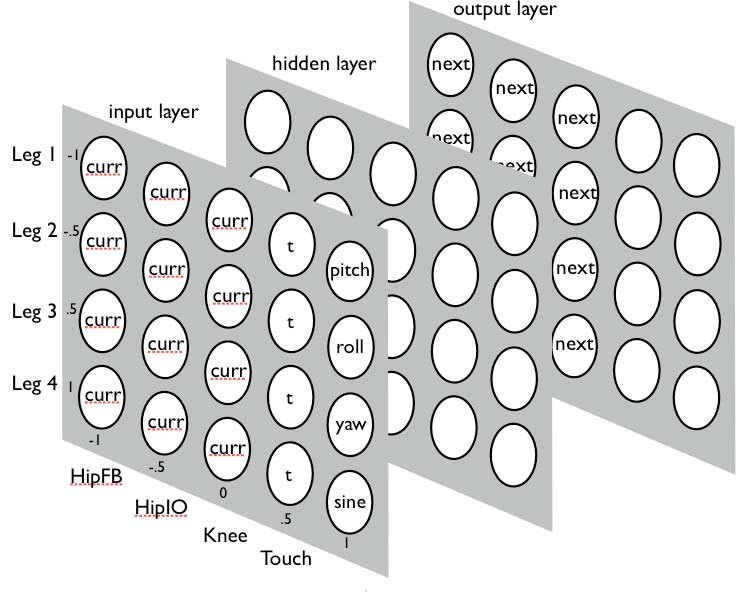
\includegraphics[width=0.4\textwidth]{clunenet}
  \end{center}
  \caption{rozložení sítě v~\cite{clunegait}, převzato \cite{clunegait}}
\end{wrapfigure}

\cite{clunegait} umisťuje do každého řádku v~\emph{substrátu} jednu nohu a do posledního sloupce přidává neuspořádaně zbývající informace (viz obr. 2).\par
\begin{wrapfigure}[10]{r}{0.59\textwidth}
  \begin{center}
    \includegraphics[width=0.58\textwidth]{sandwich}
  \end{center}
  \caption{symetrické rozložení sítě, barvy označují jednotlivé nohy, vlevo vstupní vrstva, vpravo výstupní vrstva, prostřední skrytá vrstva nevyobrazena}
\end{wrapfigure}
Tento postup sice dává geometricky najevo související buňky -- podobné informace jsou ve stejných sloupcích, ale opomíjí rozložení nohou v~prostoru, proto se v~tomto projektu používá struktura, která za pomoci symetrie dává najevo souvislosti typu \emph{přední/zadní pár nohou} a \emph{levá/pravá noha}. Pro nejlepší výsledky je v~rozložení nohou středová souměrnost a zbývající informace jsou v~prostřední řadě mezi nohama. Každá noha je popsána pomocí dvou úhlů kloubů a dotykového \emph{senzoru} na spodním článku nohy, jehož hodnota je nastavena na $-1$ bez doteku a $1$ s~dotekem, pro plynulost pohybu mají tyto hodnoty lineární přechod o~délce 25 snímků.\par
Jako přídavné proměnné jsou v~tomto rozložení $sin(t/T)$, $cos(t/T)$, kde T je experimentálně určená konstanta 40, dále úhel těla robota se zemí $\Phi$ a $1$ jakožto lineární konstanta.\par
Z~výstupní vrstvy jsou využívány pouze neurony v~pozicích úhlů nohou, které jsou převedeny na úhlovou rychlost podobně jako v~\cite{clunegait}:\\
$\omega = 4,5\cdot(\phi_{new} - \phi_{cur})$
\subsection{simulace}
K~simulaci je použita knihovna JBox2D\cite{jbox2D}. Robot se skládá z~hlavního těla, na které jsou napojeny nohy. Každá z~nich je napojena pomocí rotujícího \emph{RevoluteJointu} a stejným způsobem je napojen i spodní segment v~koleni.\par
Měření vzdálenosti probíhá 3000 snímků při 60 snímcích za sekundu a dalších 1500 snímků se čeká, jestli robot po konci měření upadne na zem. Tím se zabraňuje strategiím, kdy místo snahy o~chůzi robot pouze skočí směrem kupředu.\par
\section{Výsledky}
Nejlepším výsledkem programu je ovladač robota, který je schopen během 3000 snímků ujít 177 délkových jednotek. Je schopen dosáhnout pravidelné chůze, která vypadá stabilně a přirozeně.\par 
K~lidské, či zvířecí chůzi mu ale chybí jedna zásadní vlastnost -- při chůzi nezvedá nohy. K~tomu dochází zejména z~toho důvodu, že při chůzi na absolutně hladkém povrchu k~tomu ani není důvod a stálý kontakt se zemí mu dodává další stabilitu.\par
Jako aktivační funkce se ve výsledné neuronové síti používá sigmoida s~posunutým nulovým bodem z~0,5 na 0, čímž dosahuje hodnot od -1 do 1 a je podobná často používané hyperbolické tangentě.
Algoritmus zkonvergoval po přibližně 2000 generacích (viz obr. 4), což trvalo řádově 10 hodin na běžném laptopu (2 jádra, 2,4 GHz)
\begin{figure}[h]
\caption{graf vývoje chůze}

\begin{tikzpicture}
\begin{axis}[
    axis lines = left,
    xlabel = generace,
    ylabel = {fitness},
    width = \linewidth,
    height = 5cm
]


\addplot[
    color=blue,
%    mark=line,
    ]
    coordinates {
(0,0.001)(1,0.001)(2,0.001)(3,0.001)(4,0.001)(5,0.001)(6,0.918)(7,0.918)(8,0.918)(9,0.918)(10,1.292)(11,1.295)(12,1.354)(13,1.354)(14,1.354)(15,1.465)(16,2.158)(17,3.494)(18,3.494)(19,3.812)(20,3.812)(21,3.812)(22,4.272)(23,4.272)(24,4.272)(25,56.160)(26,62.363)(27,75.610)(28,75.610)(29,80.947)(30,80.947)(31,80.947)(32,80.947)(33,81.417)(34,83.910)(35,88.336)(36,88.336)(37,88.336)(38,88.336)(39,95.200)(40,95.200)(41,96.598)(42,96.598)(43,107.433)(44,107.433)(45,107.433)(46,107.433)(47,107.433)(48,107.433)(49,107.433)(50,107.433)(51,107.433)(52,107.433)(53,107.433)(54,107.433)(55,107.433)(56,107.433)(57,107.433)(58,107.433)(59,107.433)(60,107.433)(61,107.433)(62,107.433)(63,107.433)(64,107.433)(65,107.433)(66,107.433)(67,107.433)(68,110.037)(69,110.037)(70,110.037)(71,110.037)(72,110.037)(73,110.037)(74,110.037)(75,110.037)(76,110.037)(77,110.037)(78,110.037)(79,110.037)(80,110.037)(81,110.037)(82,110.037)(83,110.037)(84,110.037)(85,110.037)(86,110.037)(87,110.037)(88,110.037)(89,110.037)(90,110.037)(91,110.037)(92,110.037)(93,110.037)(94,110.037)(95,110.037)(96,110.037)(97,110.037)(98,110.037)(99,110.037)(100,110.037)(101,110.037)(102,110.037)(103,110.037)(104,110.037)(105,138.826)(106,138.826)(107,138.826)(108,138.826)(109,138.826)(110,138.826)(111,138.826)(112,138.826)(113,138.826)(114,138.826)(115,138.826)(116,138.826)(117,138.826)(118,138.826)(119,138.826)(120,138.826)(121,138.826)(122,138.826)(123,138.826)(124,138.826)(125,138.826)(126,138.826)(127,139.595)(128,139.595)(129,139.595)(130,139.595)(131,139.595)(132,139.595)(133,139.595)(134,139.595)(135,139.595)(136,139.595)(137,139.595)(138,139.595)(139,139.595)(140,139.595)(141,139.595)(142,139.595)(143,139.595)(144,139.595)(145,139.595)(146,139.595)(147,139.595)(148,139.595)(149,139.595)(150,139.857)(151,139.857)(152,139.857)(153,139.857)(154,139.857)(155,139.857)(156,150.317)(157,150.317)(158,150.317)(159,150.317)(160,150.317)(161,150.317)(162,150.317)(163,150.317)(164,150.317)(165,150.317)(166,150.317)(167,150.317)(168,150.317)(169,150.317)(170,150.317)(171,150.317)(172,150.317)(173,150.317)(174,150.317)(175,150.317)(176,150.317)(177,150.317)(178,150.317)(179,150.317)(180,150.317)(181,150.317)(182,150.317)(183,150.317)(184,150.317)(185,150.317)(186,150.317)(187,150.317)(188,150.317)(189,150.317)(190,150.317)(191,150.317)(192,150.317)(193,150.317)(194,150.317)(195,150.317)(196,150.317)(197,150.317)(198,150.317)(199,150.317)(200,150.317)(201,150.317)(202,150.317)(203,150.317)(204,150.317)(205,150.317)(206,150.317)(207,150.317)(208,150.317)(209,150.317)(210,150.317)(211,150.317)(212,150.317)(213,150.317)(214,150.317)(215,150.317)(216,150.317)(217,150.317)(218,150.317)(219,150.317)(220,150.317)(221,150.317)(222,150.317)(223,150.317)(224,150.317)(225,150.317)(226,150.317)(227,150.317)(228,150.317)(229,150.317)(230,150.317)(231,150.317)(232,150.317)(233,150.317)(234,150.317)(235,150.317)(236,150.317)(237,150.317)(238,150.317)(239,150.317)(240,150.317)(241,150.317)(242,150.317)(243,150.317)(244,150.317)(245,150.317)(246,150.317)(247,150.317)(248,150.317)(249,150.317)(250,150.317)(251,150.317)(252,150.317)(253,150.317)(254,150.317)(255,150.317)(256,150.317)(257,150.317)(258,150.317)(259,150.317)(260,150.317)(261,150.317)(262,150.317)(263,150.317)(264,150.317)(265,150.317)(266,150.317)(267,150.317)(268,150.317)(269,150.317)(270,150.317)(271,150.317)(272,150.317)(273,150.317)(274,150.317)(275,150.317)(276,150.317)(277,150.317)(278,150.317)(279,150.317)(280,150.317)(281,150.317)(282,150.317)(283,150.317)(284,150.317)(285,150.317)(286,150.317)(287,150.317)(288,150.317)(289,150.317)(290,150.317)(291,150.317)(292,150.317)(293,150.317)(294,150.317)(295,150.317)(296,150.317)(297,150.317)(298,150.317)(299,150.317)(300,150.317)(301,150.317)(302,150.317)(303,150.317)(304,150.317)(305,150.317)(306,150.317)(307,150.317)(308,150.317)(309,150.317)(310,150.317)(311,150.317)(312,150.317)(313,150.317)(314,150.317)(315,150.317)(316,150.317)(317,150.317)(318,150.317)(319,150.317)(320,150.317)(321,150.317)(322,150.317)(323,150.317)(324,150.317)(325,150.317)(326,150.317)(327,150.317)(328,150.317)(329,150.317)(330,150.317)(331,150.317)(332,150.317)(333,150.317)(334,150.317)(335,150.317)(336,150.317)(337,150.317)(338,150.317)(339,150.317)(340,150.317)(341,150.317)(342,150.317)(343,150.317)(344,150.317)(345,150.317)(346,150.317)(347,150.317)(348,150.317)(349,150.317)(350,150.317)(351,150.317)(352,150.317)(353,150.317)(354,150.317)(355,150.317)(356,150.317)(357,150.317)(358,150.317)(359,150.317)(360,150.317)(361,150.317)(362,150.317)(363,150.317)(364,150.317)(365,150.317)(366,150.317)(367,150.317)(368,150.317)(369,150.317)(370,150.317)(371,150.317)(372,150.317)(373,150.317)(374,150.317)(375,150.317)(376,150.317)(377,150.317)(378,150.317)(379,151.393)(380,151.393)(381,151.393)(382,151.393)(383,151.393)(384,156.473)(385,156.473)(386,156.473)(387,156.473)(388,156.473)(389,156.473)(390,156.473)(391,156.473)(392,156.473)(393,156.473)(394,156.473)(395,156.473)(396,156.473)(397,158.080)(398,158.080)(399,158.080)(400,158.080)(401,158.080)(402,158.080)(403,158.080)(404,158.080)(405,158.080)(406,158.080)(407,166.875)(408,166.875)(409,166.875)(410,168.241)(411,168.241)(412,168.241)(413,168.241)(414,168.241)(415,168.241)(416,168.241)(417,168.241)(418,168.241)(419,168.241)(420,168.241)(421,168.241)(422,168.241)(423,168.241)(424,168.241)(425,168.241)(426,168.241)(427,168.241)(428,168.381)(429,168.381)(430,168.381)(431,168.381)(432,168.381)(433,168.381)(434,168.381)(435,168.381)(436,168.381)(437,168.381)(438,168.381)(439,168.381)(440,168.381)(441,168.381)(442,168.381)(443,168.381)(444,168.381)(445,168.381)(446,168.381)(447,168.381)(448,168.381)(449,168.381)(450,168.381)(451,168.381)(452,168.381)(453,168.381)(454,168.381)(455,168.381)(456,168.381)(457,168.381)(458,168.381)(459,168.381)(460,168.381)(461,168.381)(462,168.381)(463,168.381)(464,168.381)(465,168.381)(466,168.381)(467,168.381)(468,168.381)(469,168.381)(470,168.381)(471,168.381)(472,168.381)(473,168.381)(474,168.381)(475,168.381)(476,168.381)(477,168.381)(478,168.381)(479,168.381)(480,168.381)(481,168.381)(482,168.381)(483,168.381)(484,168.381)(485,168.381)(486,168.381)(487,168.381)(488,168.381)(489,168.381)(490,168.381)(491,168.381)(492,171.982)(493,171.982)(494,171.982)(495,171.982)(496,171.982)(497,171.982)(498,171.982)(499,171.982)(500,171.982)(501,171.982)(502,171.982)(503,171.982)(504,171.982)(505,171.982)(506,171.982)(507,171.982)(508,171.982)(509,171.982)(510,171.982)(511,171.982)(512,171.982)(513,171.982)(514,171.982)(515,171.982)(516,171.982)(517,171.982)(518,171.982)(519,171.982)(520,171.982)(521,171.982)(522,171.982)(523,171.982)(524,171.982)(525,171.982)(526,171.982)(527,171.982)(528,171.982)(529,171.982)(530,171.982)(531,171.982)(532,171.982)(533,171.982)(534,171.982)(535,171.982)(536,171.982)(537,171.982)(538,171.982)(539,171.982)(540,171.982)(541,171.982)(542,171.982)(543,171.982)(544,171.982)(545,171.982)(546,171.982)(547,171.982)(548,171.982)(549,171.982)(550,171.982)(551,171.982)(552,171.982)(553,171.982)(554,171.982)(555,171.982)(556,171.982)(557,171.982)(558,171.982)(559,171.982)(560,171.982)(561,171.982)(562,171.982)(563,171.982)(564,171.982)(565,171.982)(566,171.982)(567,171.982)(568,171.982)(569,171.982)(570,171.982)(571,171.982)(572,171.982)(573,171.982)(574,171.982)(575,171.982)(576,171.982)(577,171.982)(578,171.982)(579,171.982)(580,171.982)(581,171.982)(582,171.982)(583,171.982)(584,171.982)(585,171.982)(586,171.982)(587,171.982)(588,171.982)(589,171.982)(590,171.982)(591,171.982)(592,171.982)(593,171.982)(594,171.982)(595,171.982)(596,171.982)(597,171.982)(598,171.982)(599,171.982)(600,171.982)(601,171.982)(602,171.982)(603,171.982)(604,171.982)(605,171.982)(606,171.982)(607,171.982)(608,171.982)(609,171.982)(610,172.782)(611,172.782)(612,172.782)(613,172.782)(614,172.782)(615,172.782)(616,172.782)(617,172.782)(618,172.782)(619,172.782)(620,172.782)(621,172.782)(622,172.782)(623,172.782)(624,172.782)(625,172.782)(626,172.782)(627,172.782)(628,172.782)(629,172.782)(630,172.782)(631,172.782)(632,172.782)(633,172.782)(634,172.782)(635,172.782)(636,172.782)(637,172.782)(638,172.782)(639,172.782)(640,172.782)(641,172.782)(642,172.782)(643,172.782)(644,172.782)(645,172.782)(646,172.782)(647,172.782)(648,172.782)(649,172.782)(650,172.782)(651,172.782)(652,172.782)(653,172.782)(654,172.782)(655,172.782)(656,172.782)(657,172.782)(658,172.782)(659,172.782)(660,172.782)(661,172.782)(662,172.782)(663,172.782)(664,172.782)(665,172.782)(666,172.782)(667,172.782)(668,172.782)(669,172.782)(670,172.782)(671,172.782)(672,172.782)(673,172.782)(674,172.782)(675,172.782)(676,172.782)(677,172.782)(678,172.782)(679,172.782)(680,172.782)(681,172.782)(682,172.782)(683,172.782)(684,172.782)(685,172.782)(686,172.782)(687,172.782)(688,172.782)(689,172.782)(690,172.782)(691,172.782)(692,172.782)(693,172.782)(694,172.782)(695,172.782)(696,172.782)(697,172.782)(698,172.782)(699,172.782)(700,172.782)(701,172.782)(702,172.782)(703,172.782)(704,172.782)(705,172.782)(706,172.782)(707,172.782)(708,172.782)(709,172.782)(710,172.782)(711,172.782)(712,172.782)(713,172.782)(714,172.782)(715,172.782)(716,172.782)(717,172.782)(718,172.782)(719,172.782)(720,172.782)(721,172.782)(722,172.782)(723,172.782)(724,172.782)(725,172.782)(726,172.782)(727,172.782)(728,172.782)(729,172.782)(730,172.782)(731,172.782)(732,172.782)(733,172.782)(734,172.782)(735,172.782)(736,172.782)(737,172.782)(738,172.782)(739,172.782)(740,172.782)(741,172.782)(742,172.782)(743,172.782)(744,172.782)(745,172.782)(746,172.782)(747,172.782)(748,172.782)(749,172.782)(750,172.782)(751,172.782)(752,172.782)(753,172.782)(754,172.782)(755,172.782)(756,172.782)(757,172.782)(758,172.782)(759,172.782)(760,172.782)(761,172.782)(762,172.782)(763,172.782)(764,172.782)(765,172.782)(766,172.782)(767,172.782)(768,172.782)(769,172.782)(770,172.782)(771,172.782)(772,172.782)(773,172.782)(774,172.782)(775,172.782)(776,172.782)(777,172.782)(778,172.782)(779,172.782)(780,172.782)(781,172.782)(782,172.782)(783,172.782)(784,172.782)(785,172.782)(786,172.782)(787,172.782)(788,172.782)(789,172.782)(790,172.782)(791,172.782)(792,172.782)(793,172.782)(794,172.782)(795,172.782)(796,172.782)(797,172.782)(798,172.782)(799,172.782)(800,172.782)(801,172.782)(802,172.782)(803,172.782)(804,172.782)(805,172.782)(806,172.782)(807,172.782)(808,172.782)(809,172.782)(810,172.782)(811,172.782)(812,172.782)(813,172.782)(814,172.782)(815,172.782)(816,172.782)(817,172.782)(818,172.782)(819,172.782)(820,172.782)(821,172.782)(822,172.782)(823,172.782)(824,172.782)(825,172.782)(826,172.782)(827,172.782)(828,172.782)(829,172.782)(830,172.782)(831,172.782)(832,172.782)(833,172.782)(834,172.782)(835,172.782)(836,172.782)(837,172.782)(838,172.782)(839,172.782)(840,172.782)(841,172.782)(842,172.782)(843,172.782)(844,172.782)(845,172.782)(846,172.782)(847,172.782)(848,172.782)(849,172.782)(850,172.782)(851,172.782)(852,172.782)(853,172.782)(854,172.782)(855,172.782)(856,172.782)(857,172.782)(858,172.782)(859,172.782)(860,172.782)(861,172.782)(862,172.782)(863,172.782)(864,172.782)(865,172.782)(866,172.782)(867,172.782)(868,172.782)(869,172.782)(870,172.782)(871,172.782)(872,172.782)(873,172.782)(874,172.782)(875,172.782)(876,172.782)(877,172.782)(878,172.782)(879,172.782)(880,172.782)(881,172.782)(882,172.782)(883,172.782)(884,172.782)(885,172.782)(886,172.782)(887,172.782)(888,172.782)(889,172.782)(890,172.782)(891,172.782)(892,172.782)(893,172.782)(894,172.782)(895,172.782)(896,172.782)(897,172.782)(898,172.782)(899,172.782)(900,172.782)(901,172.782)(902,172.782)(903,172.782)(904,172.782)(905,172.782)(906,172.782)(907,172.782)(908,172.782)(909,172.782)(910,172.782)(911,172.782)(912,172.782)(913,172.782)(914,172.782)(915,172.782)(916,172.782)(917,172.782)(918,172.782)(919,172.782)(920,172.782)(921,172.782)(922,172.782)(923,172.782)(924,172.782)(925,172.782)(926,172.782)(927,172.782)(928,172.782)(929,172.782)(930,172.782)(931,172.782)(932,172.782)(933,172.782)(934,172.782)(935,172.782)(936,172.782)(937,172.782)(938,172.782)(939,172.782)(940,172.782)(941,172.782)(942,172.782)(943,172.782)(944,172.782)(945,172.782)(946,172.782)(947,172.782)(948,172.782)(949,172.782)(950,172.782)(951,172.782)(952,172.782)(953,172.782)(954,172.782)(955,172.782)(956,172.782)(957,172.782)(958,172.782)(959,172.782)(960,172.782)(961,172.782)(962,172.782)(963,172.782)(964,172.782)(965,172.782)(966,172.782)(967,172.782)(968,172.782)(969,172.782)(970,172.782)(971,172.782)(972,172.782)(973,172.782)(974,172.782)(975,172.782)(976,172.782)(977,172.782)(978,172.782)(979,172.782)(980,172.782)(981,172.782)(982,172.782)(983,172.782)(984,172.782)(985,172.782)(986,172.782)(987,172.782)(988,172.782)(989,172.782)(990,172.782)(991,172.782)(992,172.782)(993,172.782)(994,172.782)(995,172.782)(996,172.782)(997,172.782)(998,172.782)(999,172.782)(1000,172.782)(1001,172.782)(1002,172.782)(1003,172.782)(1004,172.782)(1005,172.782)(1006,172.782)(1007,172.782)(1008,172.782)(1009,172.782)(1010,172.782)(1011,172.782)(1012,172.782)(1013,172.782)(1014,172.782)(1015,172.782)(1016,172.782)(1017,172.782)(1018,172.782)(1019,172.782)(1020,172.782)(1021,172.782)(1022,172.782)(1023,172.782)(1024,172.782)(1025,172.782)(1026,172.782)(1027,172.782)(1028,172.782)(1029,172.782)(1030,172.782)(1031,172.782)(1032,172.782)(1033,172.782)(1034,172.782)(1035,172.782)(1036,172.782)(1037,172.782)(1038,172.782)(1039,172.782)(1040,172.782)(1041,172.782)(1042,172.782)(1043,172.782)(1044,172.782)(1045,172.782)(1046,172.782)(1047,172.782)(1048,172.782)(1049,172.782)(1050,172.782)(1051,172.782)(1052,172.782)(1053,172.782)(1054,172.782)(1055,172.782)(1056,172.782)(1057,172.782)(1058,172.782)(1059,172.782)(1060,172.782)(1061,172.782)(1062,172.782)(1063,172.782)(1064,172.782)(1065,172.782)(1066,172.782)(1067,172.782)(1068,172.782)(1069,172.782)(1070,172.782)(1071,172.782)(1072,172.782)(1073,172.782)(1074,172.782)(1075,172.782)(1076,172.782)(1077,172.782)(1078,172.782)(1079,172.782)(1080,172.782)(1081,172.782)(1082,172.782)(1083,172.782)(1084,173.840)(1085,173.840)(1086,173.840)(1087,173.840)(1088,173.840)(1089,173.840)(1090,173.840)(1091,173.840)(1092,173.840)(1093,173.840)(1094,173.840)(1095,173.840)(1096,173.840)(1097,173.840)(1098,173.840)(1099,173.840)(1100,173.840)(1101,173.840)(1102,173.840)(1103,173.840)(1104,173.840)(1105,173.840)(1106,173.840)(1107,173.840)(1108,173.840)(1109,173.840)(1110,173.840)(1111,173.840)(1112,173.840)(1113,173.840)(1114,173.840)(1115,173.840)(1116,173.840)(1117,173.840)(1118,173.840)(1119,173.840)(1120,173.840)(1121,173.840)(1122,173.840)(1123,173.840)(1124,173.840)(1125,173.840)(1126,173.840)(1127,173.840)(1128,173.840)(1129,173.840)(1130,173.840)(1131,173.840)(1132,173.840)(1133,173.840)(1134,173.840)(1135,173.840)(1136,173.840)(1137,173.840)(1138,173.840)(1139,173.840)(1140,173.840)(1141,173.840)(1142,173.840)(1143,173.840)(1144,173.840)(1145,173.840)(1146,173.840)(1147,173.840)(1148,173.840)(1149,173.840)(1150,173.840)(1151,173.840)(1152,173.840)(1153,173.840)(1154,173.840)(1155,173.840)(1156,173.840)(1157,173.840)(1158,173.840)(1159,173.840)(1160,173.840)(1161,173.840)(1162,173.840)(1163,173.840)(1164,173.840)(1165,173.840)(1166,173.840)(1167,173.840)(1168,173.840)(1169,173.840)(1170,173.840)(1171,173.840)(1172,173.840)(1173,173.840)(1174,173.840)(1175,173.840)(1176,173.840)(1177,173.840)(1178,173.840)(1179,173.840)(1180,173.840)(1181,173.840)(1182,173.840)(1183,173.840)(1184,173.840)(1185,173.840)(1186,173.840)(1187,173.840)(1188,173.840)(1189,173.840)(1190,173.840)(1191,173.840)(1192,173.840)(1193,173.840)(1194,173.840)(1195,173.840)(1196,173.840)(1197,173.840)(1198,173.840)(1199,173.840)(1200,173.840)(1201,173.840)(1202,173.840)(1203,173.840)(1204,173.840)(1205,173.840)(1206,173.840)(1207,173.840)(1208,173.840)(1209,173.840)(1210,173.840)(1211,173.840)(1212,173.840)(1213,173.840)(1214,173.840)(1215,173.840)(1216,173.840)(1217,173.840)(1218,173.840)(1219,173.840)(1220,173.840)(1221,173.840)(1222,173.840)(1223,173.840)(1224,173.840)(1225,173.840)(1226,173.840)(1227,173.840)(1228,173.840)(1229,173.840)(1230,173.840)(1231,173.840)(1232,173.840)(1233,173.840)(1234,173.840)(1235,173.840)(1236,173.840)(1237,173.840)(1238,173.840)(1239,173.840)(1240,173.840)(1241,173.840)(1242,173.840)(1243,173.840)(1244,173.840)(1245,173.840)(1246,173.840)(1247,173.840)(1248,173.840)(1249,173.840)(1250,173.840)(1251,173.840)(1252,173.840)(1253,173.840)(1254,173.840)(1255,173.840)(1256,173.840)(1257,173.840)(1258,173.840)(1259,173.840)(1260,173.840)(1261,173.840)(1262,173.840)(1263,173.840)(1264,173.840)(1265,173.840)(1266,173.840)(1267,173.840)(1268,173.840)(1269,173.840)(1270,173.840)(1271,173.840)(1272,173.840)(1273,173.840)(1274,173.840)(1275,173.840)(1276,173.840)(1277,173.840)(1278,173.840)(1279,173.840)(1280,173.840)(1281,173.840)(1282,173.840)(1283,173.840)(1284,173.840)(1285,173.840)(1286,173.840)(1287,173.840)(1288,173.840)(1289,173.840)(1290,173.840)(1291,173.840)(1292,173.840)(1293,173.840)(1294,173.840)(1295,173.840)(1296,173.840)(1297,173.840)(1298,173.840)(1299,173.840)(1300,173.840)(1301,173.840)(1302,173.840)(1303,173.840)(1304,173.840)(1305,173.840)(1306,173.840)(1307,173.840)(1308,173.840)(1309,173.840)(1310,173.840)(1311,173.840)(1312,173.840)(1313,173.840)(1314,173.840)(1315,173.840)(1316,173.840)(1317,173.840)(1318,173.840)(1319,173.840)(1320,173.840)(1321,173.840)(1322,173.840)(1323,173.840)(1324,173.840)(1325,173.840)(1326,173.840)(1327,173.840)(1328,173.840)(1329,173.840)(1330,174.347)(1331,174.347)(1332,174.347)(1333,174.347)(1334,174.347)(1335,174.347)(1336,174.347)(1337,174.347)(1338,174.347)(1339,174.347)(1340,174.347)(1341,174.347)(1342,174.347)(1343,174.347)(1344,174.347)(1345,174.347)(1346,174.347)(1347,174.347)(1348,174.347)(1349,174.347)(1350,174.347)(1351,174.347)(1352,174.347)(1353,174.347)(1354,174.347)(1355,174.347)(1356,174.347)(1357,174.347)(1358,174.347)(1359,174.347)(1360,174.347)(1361,174.347)(1362,174.347)(1363,174.347)(1364,174.347)(1365,174.347)(1366,174.347)(1367,174.347)(1368,174.347)(1369,174.347)(1370,174.347)(1371,174.347)(1372,174.347)(1373,174.347)(1374,174.347)(1375,174.347)(1376,174.347)(1377,174.347)(1378,174.347)(1379,174.347)(1380,174.347)(1381,174.347)(1382,174.347)(1383,174.347)(1384,174.347)(1385,174.347)(1386,174.347)(1387,174.347)(1388,174.347)(1389,174.347)(1390,174.347)(1391,174.347)(1392,174.347)(1393,174.347)(1394,174.347)(1395,174.347)(1396,174.347)(1397,174.347)(1398,174.347)(1399,174.347)(1400,174.347)(1401,174.347)(1402,174.347)(1403,174.347)(1404,174.347)(1405,174.347)(1406,174.347)(1407,174.347)(1408,174.347)(1409,174.347)(1410,174.347)(1411,174.347)(1412,174.347)(1413,174.347)(1414,174.347)(1415,174.347)(1416,174.347)(1417,174.347)(1418,174.347)(1419,174.347)(1420,174.347)(1421,174.347)(1422,174.347)(1423,174.347)(1424,174.347)(1425,174.347)(1426,174.347)(1427,174.347)(1428,174.347)(1429,174.347)(1430,174.347)(1431,174.347)(1432,174.347)(1433,174.347)(1434,174.347)(1435,174.347)(1436,174.347)(1437,174.347)(1438,174.347)(1439,174.347)(1440,174.347)(1441,174.347)(1442,174.347)(1443,174.347)(1444,174.347)(1445,174.347)(1446,174.347)(1447,174.347)(1448,174.347)(1449,174.347)(1450,174.347)(1451,174.347)(1452,174.347)(1453,174.347)(1454,174.347)(1455,174.347)(1456,174.347)(1457,174.347)(1458,174.347)(1459,174.347)(1460,174.347)(1461,174.347)(1462,174.347)(1463,174.347)(1464,174.347)(1465,174.347)(1466,174.347)(1467,174.347)(1468,174.347)(1469,174.347)(1470,174.347)(1471,174.347)(1472,174.347)(1473,174.347)(1474,174.347)(1475,174.347)(1476,174.347)(1477,174.347)(1478,174.347)(1479,174.347)(1480,174.347)(1481,174.347)(1482,174.347)(1483,174.347)(1484,174.347)(1485,174.347)(1486,174.347)(1487,174.347)(1488,174.347)(1489,174.347)(1490,174.347)(1491,174.347)(1492,174.347)(1493,174.347)(1494,174.347)(1495,174.347)(1496,174.347)(1497,174.347)(1498,174.347)(1499,174.347)(1500,174.347)(1501,174.347)(1502,174.347)(1503,174.347)(1504,174.347)(1505,174.347)(1506,174.347)(1507,174.347)(1508,174.347)(1509,174.347)(1510,174.347)(1511,174.347)(1512,174.347)(1513,174.347)(1514,174.347)(1515,174.347)(1516,174.347)(1517,174.347)(1518,174.347)(1519,174.347)(1520,174.347)(1521,174.347)(1522,174.347)(1523,174.347)(1524,174.347)(1525,174.347)(1526,174.347)(1527,174.347)(1528,174.347)(1529,174.347)(1530,174.347)(1531,174.347)(1532,174.347)(1533,174.347)(1534,174.347)(1535,174.347)(1536,174.347)(1537,174.347)(1538,174.347)(1539,174.347)(1540,174.347)(1541,174.347)(1542,174.347)(1543,174.347)(1544,174.347)(1545,174.347)(1546,174.347)(1547,174.347)(1548,174.347)(1549,174.347)(1550,174.347)(1551,174.347)(1552,174.347)(1553,174.347)(1554,174.347)(1555,174.347)(1556,174.347)(1557,174.347)(1558,174.347)(1559,174.347)(1560,174.347)(1561,174.347)(1562,174.347)(1563,174.347)(1564,174.347)(1565,174.347)(1566,174.347)(1567,174.347)(1568,174.347)(1569,174.347)(1570,174.347)(1571,174.347)(1572,174.347)(1573,174.347)(1574,174.347)(1575,174.347)(1576,174.347)(1577,174.347)(1578,174.347)(1579,174.347)(1580,174.347)(1581,174.347)(1582,174.347)(1583,174.347)(1584,174.347)(1585,174.347)(1586,174.347)(1587,174.347)(1588,174.347)(1589,174.347)(1590,174.347)(1591,174.347)(1592,174.347)(1593,174.347)(1594,174.347)(1595,174.347)(1596,174.347)(1597,174.347)(1598,174.347)(1599,174.347)(1600,174.347)(1601,174.347)(1602,174.347)(1603,174.347)(1604,174.347)(1605,174.347)(1606,174.347)(1607,174.347)(1608,174.347)(1609,174.347)(1610,176.091)(1611,176.091)(1612,176.091)(1613,176.091)(1614,176.091)(1615,176.091)(1616,176.091)(1617,176.091)(1618,176.091)(1619,176.091)(1620,176.091)(1621,176.091)(1622,176.091)(1623,176.091)(1624,176.091)(1625,176.091)(1626,176.091)(1627,176.091)(1628,176.091)(1629,176.091)(1630,176.091)(1631,176.091)(1632,176.091)(1633,176.091)(1634,177.066)(1635,177.066)(1636,177.066)(1637,177.066)(1638,177.066)(1639,177.066)(1640,177.066)(1641,177.066)(1642,177.066)(1643,177.066)(1644,177.066)(1645,177.066)(1646,177.066)(1647,177.066)(1648,177.066)(1649,177.066)(1650,177.066)(1651,177.066)(1652,177.066)(1653,177.066)(1654,177.066)(1655,177.066)(1656,177.066)(1657,177.066)(1658,177.066)(1659,177.066)(1660,177.066)(1661,177.066)(1662,177.066)(1663,177.066)(1664,177.066)(1665,177.066)(1666,177.066)(1667,177.066)(1668,177.066)(1669,177.066)(1670,177.066)(1671,177.066)(1672,177.066)(1673,177.066)(1674,177.066)(1675,177.066)(1676,177.066)(1677,177.066)(1678,177.066)(1679,177.066)(1680,177.066)(1681,177.066)(1682,177.066)(1683,177.066)(1684,177.066)(1685,177.066)(1686,177.066)(1687,177.066)(1688,177.066)(1689,177.066)(1690,177.066)(1691,177.066)(1692,177.066)(1693,177.066)(1694,177.066)(1695,177.066)(1696,177.066)(1697,177.066)(1698,177.066)(1699,177.066)(1700,177.066)(1701,177.066)(1702,177.066)(1703,177.066)(1704,177.066)(1705,177.066)(1706,177.066)(1707,177.066)(1708,177.066)(1709,177.066)(1710,177.066)(1711,177.066)(1712,177.066)(1713,177.066)(1714,177.066)(1715,177.066)(1716,177.066)(1717,177.066)(1718,177.066)(1719,177.066)(1720,177.066)(1721,177.066)(1722,177.066)(1723,177.066)(1724,177.066)(1725,177.066)(1726,177.066)(1727,177.066)(1728,177.066)(1729,177.066)(1730,177.066)(1731,177.066)(1732,177.066)(1733,177.066)(1734,177.066)(1735,177.066)(1736,177.066)(1737,177.066)(1738,177.066)(1739,177.066)(1740,177.066)(1741,177.066)(1742,177.066)(1743,177.066)(1744,177.066)(1745,177.066)(1746,177.066)(1747,177.066)(1748,177.066)(1749,177.066)(1750,177.066)(1751,177.066)(1752,177.066)(1753,177.066)(1754,177.066)(1755,177.066)(1756,177.066)(1757,177.066)(1758,177.066)(1759,177.066)(1760,177.066)(1761,177.066)(1762,177.066)(1763,177.066)(1764,177.066)(1765,177.066)(1766,177.066)(1767,177.066)(1768,177.066)(1769,177.066)(1770,177.066)(1771,177.066)(1772,177.066)(1773,177.066)(1774,177.066)(1775,177.066)(1776,177.066)(1777,177.066)(1778,177.066)(1779,177.066)(1780,177.066)(1781,177.066)(1782,177.066)(1783,177.066)(1784,177.066)(1785,177.066)(1786,177.066)(1787,177.066)(1788,177.066)(1789,177.066)(1790,177.066)(1791,177.066)(1792,177.066)(1793,177.066)(1794,177.066)(1795,177.066)(1796,177.066)(1797,177.066)(1798,177.066)(1799,177.066)(1800,177.066)(1801,177.066)(1802,177.066)(1803,177.066)(1804,177.066)(1805,177.066)(1806,177.066)(1807,177.066)(1808,177.066)(1809,177.066)(1810,177.066)(1811,177.066)(1812,177.066)(1813,177.066)(1814,177.066)(1815,177.066)(1816,177.066)(1817,177.066)(1818,177.066)(1819,177.066)(1820,177.066)(1821,177.066)(1822,177.066)(1823,177.066)(1824,177.066)(1825,177.066)(1826,177.066)(1827,177.066)(1828,177.066)(1829,177.066)(1830,177.066)(1831,177.066)(1832,177.066)(1833,177.066)(1834,177.066)(1835,177.066)(1836,177.066)(1837,177.066)(1838,177.066)(1839,177.066)(1840,177.066)(1841,177.066)(1842,177.066)(1843,177.066)(1844,177.066)(1845,177.066)(1846,177.066)(1847,177.066)(1848,177.066)(1849,177.066)(1850,177.066)(1851,177.066)(1852,177.066)(1853,177.066)(1854,177.066)(1855,177.066)(1856,177.066)(1857,177.066)(1858,177.066)(1859,177.066)(1860,177.066)(1861,177.066)(1862,177.066)(1863,177.066)(1864,177.066)(1865,177.066)(1866,177.066)(1867,177.066)(1868,177.066)(1869,177.066)(1870,177.066)(1871,177.066)(1872,177.066)(1873,177.066)(1874,177.066)(1875,177.066)(1876,177.066)(1877,177.066)(1878,177.066)(1879,177.066)(1880,177.066)(1881,177.066)(1882,177.066)(1883,177.066)(1884,177.066)(1885,177.066)(1886,177.066)(1887,177.066)(1888,177.066)(1889,177.066)(1890,177.066)(1891,177.066)(1892,177.066)(1893,177.066)(1894,177.066)(1895,177.066)(1896,177.066)(1897,177.066)(1898,177.066)(1899,177.066)(1900,177.066)(1901,177.066)(1902,177.066)(1903,177.066)(1904,177.066)(1905,177.066)(1906,177.066)(1907,177.066)(1908,177.066)(1909,177.066)(1910,177.066)(1911,177.066)(1912,177.066)(1913,177.066)(1914,177.066)(1915,177.066)(1916,177.066)(1917,177.066)(1918,177.066)(1919,177.066)(1920,177.066)(1921,177.066)(1922,177.066)(1923,177.066)(1924,177.066)(1925,177.066)(1926,177.066)(1927,177.066)(1928,177.066)(1929,177.066)(1930,177.066)(1931,177.066)(1932,177.066)(1933,177.066)(1934,177.066)(1935,177.066)(1936,177.066)(1937,177.066)(1938,177.066)(1939,177.066)(1940,177.066)(1941,177.066)(1942,177.066)(1943,177.066)(1944,177.066)(1945,177.066)(1946,177.066)(1947,177.066)(1948,177.066)(1949,177.066)(1950,177.066)(1951,177.066)(1952,177.066)(1953,177.066)(1954,177.066)(1955,177.066)(1956,177.066)(1957,177.066)(1958,177.066)(1959,177.066)(1960,177.066)(1961,177.066)(1962,177.066)(1963,177.066)(1964,177.066)(1965,177.066)(1966,177.066)(1967,177.066)(1968,177.066)(1969,177.066)(1970,177.066)(1971,177.066)(1972,177.066)(1973,177.066)(1974,177.066)(1975,177.066)(1976,177.066)(1977,177.066)(1978,177.066)(1979,177.066)(1980,177.066)(1981,177.066)(1982,177.066)(1983,177.066)(1984,177.066)(1985,177.066)(1986,177.066)(1987,177.066)(1988,177.066)(1989,177.066)(1990,177.066)(1991,177.066)(1992,177.066)(1993,177.066)(1994,177.066)(1995,177.066)(1996,177.066)(1997,177.066)(1998,177.066)(1999,177.066)
    };
 
 
\end{axis}
\end{tikzpicture}


\end{figure}
\section{Uživatelská příručka}
Výsledkem projektu jsou dva spustitelné programy -- jeden, který provádí samotnou evoluci a druhý na zobrazovnání výsledků. Oba programy jsou napsány v~jazyce Java a lze je zkompilovat pomocí prostředí IntelliJ IDEA, ve kterém byl projekt vyvíjen. Ke kompilaci je potřeba JDK s~balíkem JavaFX (distribuce typu OpenJDK apod. nelze použít). Projekt byl vždy kompilován a spouštěn na systému Linux (Manjaro Linux s~prostředím i3wm), případná kompatibilita s~jinými systémy je pravděpodobná, avšak nezaručená.\par
\subsection{Zobrazovač výsledků}
Jedním z~programů je aplikace na zobrazování simulací výsledných sítí. Její grafické prostředí je ovládané poměrně intuitivně, v~levé části je na výběr postupně:
\begin{itemize}
\item{běh programu (podle názvu složky)}
\item{generace programu}
\item{jedinec z~generace}
\end{itemize}
Na pravé straně se zobrazuje simulace společně s~užitečnými daty umístěnými v~levé části simulačního panelu:
\begin{itemize}
\item{souřadnice $x$ těla robota}
\item{maximální dosažená souřadnice $x$ těla robota v~současné simulaci}
\item{maximální dosažená souřadnice $x$ těla robota po 3000 snímků}
\item{počet uběhlých snímků}
\item{souřadnice $y$ těla robota}
\item{současné hodnoty vstupní vrstvy neuronové sítě}
\item{současné hodnoty skryté vrstvy neuronové sítě}
\item{současné hodnoty výstupní vrstvy neuronové sítě}
\end{itemize}
Napravo od užitečných dat je vyobrazena CPPN síť. Vstupní neurony jsou na jejím levém okraji, výstupní neurony na pravém okraji, mezi nimi jsou náhodně rozloženy skryté neurony, jejichž barva značí použitou aktivační funkci. Spoje v~síti mají svůj cílový neuron označený kratším obarveným koncem. Neaktivní spoje jsou vyznačeny šedou barvou.
\subsection{Evoluční program}
Evoluční program je nutno spustit z~konzole a vyžaduje soubor \emph{config.cfg}, který obsahuje nastavení několika konstant, které lze měnit. Program ukládá výsledky do složky \emph{results}, kam také ukládá záznam průběhu programu, který rovněž vypisuje do konzole. Vypisuje několik důležitých informací, jako nejdelší dosaženou vzdálenost, počet potomků, popis jednotlivých druhů apod.
\section{Závěr} 
Výsledky ukázaly, že pro robotickou chůzi je neuroevoluční algoritmus srovnatelný s~konvenčními metodami. Program by měl být schopný generovat podobné výsledky i pro mírně odlišné konfigurace robota jen s~minimálními úpravami. I~s~výkonem běžně dostupného hardwaru se podařilo dosáhnout chůze podobné lidské či zvířecí. \par Model však byl velmi přibližný a pro reálné využití tohoto postupu by bylo nutné simulovat v~trojrozměrném prostoru a učit robota i chůzi terénem za pomoci dalších senzorů.
\begin{thebibliography}{8}
\bibitem{bostondynamics}
Introducing Spot. In: \textit{Youtube} [online]. 9.2.2015 [cit. 2017-03-20]. Dostupné z: https://www.youtube.com/watch?v=M8YjvHYbZ9w. Kanál uživatele Boston Dynamics
\bibitem{bdpaper}RAIBERT, Marc, Kevin BLANKESPOOR, Gabriel NELSON a Rob PLAYTER. \textit{BigDog, the Rough-Terrain Quadruped Robot} [online]. [cit. 2017-03-20]. DOI: 10.3182/20080706-5-KR-1001.01833. ISBN 10.3182/20080706-5-KR-1001.01833. Dostupné z: http://linkinghub.elsevier.com/retrieve/pii/S1474667016407020
\bibitem{clunegait}
CLUNE, Jeff, Benjamin E. BECKMANN, Charles OFRIA a Robert T. PENNOCK. Evolving coordinated quadruped gaits with the HyperNEAT generative encoding. In: \textit{2009 IEEE Congress on Evolutionary Computation}. IEEE, 2009, s. 2764-2771. DOI: 10.1109/CEC.2009.4983289. ISBN 978-1-4244-2958-5. Dostupné také z: http://ieeexplore.ieee.org/document/4983289/
\bibitem{neuron}
Artificial neuron. In: \textit{Wikipedia: the free encyclopedia} [online]. San Francisco (CA): Wikimedia Foundation, 2001-2017 [cit. 2017-03-21]. Dostupné z: https://en.wikipedia.org/wiki/Artificial\_neuron
\bibitem{neat}
STANLEY, Kenneth O. a Risto MIIKKULAINEN. Evolving Neural Networks through Augmenting Topologies. \emph{Evolutionary Computation} [online]. 2002, \textbf{10}(2), 99-127 [cit. 2017-03-21]. DOI: 10.1162/106365602320169811. ISSN 1063-6560. Dostupné z: http://www.mitpressjournals.org/doi/10.1162/106365602320169811
\bibitem{cppn-neat}
STANLEY, Kenneth O. Compositional pattern producing networks: A~novel abstraction of development. \emph{Genetic Programming and Evolvable Machines} [online]. 2007-6-6, \textbf{8}(2), 131-162 [cit. 2017-03-21]. DOI: 10.1007/s10710-007-9028-8. ISSN 1389-2576. Dostupné z: http://link.springer.com/10.1007/s10710-007-9028-8
\bibitem{hyperneat}
STANLEY, Kenneth O., David B. D'AMBROSIO a Jason GAUCI. A~Hypercube-Based Encoding for Evolving Large-Scale Neural Networks. \textit{Artificial Life} [online]. 2009, \textbf{15}(2), 185-212 [cit. 2017-03-21]. DOI: 10.1162/artl.2009.15.2.15202. ISSN 1064-5462. Dostupné z: http://www.mitpressjournals.org/doi/10.1162/artl.2009.15.2.15202
\bibitem{jbox2D}
\textit{JBox2D} [online]. Daniel Murphy, 2014 [cit. 2017-03-22]. Dostupné z: http://www.jbox2d.org/
\end{thebibliography}
\end{document}